\chapter{Polymers: Synthesis, Structure and Properties}\label{ch:b2:polymer-synthesis}

Nylon stockings went on sale in 1939. They came out of a laboratory that had set out, a few years
earlier, to understand how small molecules join into long ones, and that had learnt along the way a
lesson that surprises every chemist the first time: for a \omterm{def:b2:polymer-synthesis:polymer}{polymer} made by linking molecules end to end,
a 99~\% yield is not enough. This chapter explains why, describes the two ways in which chains grow,
and connects the structure of the chains to the properties of the materials.
% ledger: hist:nylon-production-1939

\begin{recall}
The school volume: \omterm{def:b2:polymer-synthesis:polymer}{polymers}, \omterm{def:b2:polymer-synthesis:polymer}{monomers} and \omterm{def:b2:polymer-synthesis:polymer}{repeat units}, addition and condensation \omterm{def:b2:polymer-synthesis:polymer}{polymers},
thermoplastics and thermosets. The Year 1 volume: radicals and homolysis, carbocations and
carbanions, the steady-state approximation. \Cref{ch:b2:acyl-substitution}: esters and amides.
\Cref{ch:b2:catalytic-cycles}: insertion into a metal--carbon bond.
\end{recall}

\section{Chains and their molar masses}

\begin{definition}[Polymer]\label{def:b2:polymer-synthesis:polymer}
A \emph{polymer}\index{polymer} is a substance made of macromolecules, each built by the repeated
linking of small molecules, the \emph{monomers}\index{monomer}. The \emph{repeat unit}\index{repeat unit}
is the smallest group of atoms whose repetition makes up the chain; the \emph{degree of
polymerisation}\index{degree of polymerisation} $X$ of a chain is the number of monomer-derived units
it contains.
\end{definition}

A sample of a synthetic \omterm{def:b2:polymer-synthesis:polymer}{polymer} is never made of identical chains: it is a mixture of chains of
different lengths, and its molar mass is an average, which depends on how the chains are counted.

\begin{definition}[Molar-mass averages]\label{def:b2:polymer-synthesis:averages}
For a sample containing $N_i$ chains of molar mass $M_i$, the \emph{number-average molar
mass}\index{number-average molar mass} and the \emph{mass-average molar mass}\index{mass-average molar mass}
are
\begin{equation*}
\bar M_n = \frac{\sum_i N_i M_i}{\sum_i N_i}, \qquad
\bar M_w = \frac{\sum_i N_i M_i^2}{\sum_i N_i M_i} = \sum_i w_i M_i,
\end{equation*}
where $w_i$ is the mass fraction of the chains of mass $M_i$. The \emph{dispersity}\index{dispersity}
$\text{\DH} = \bar M_w/\bar M_n$ is at least 1, and equal to 1 only if all chains have the same
mass. The averages $\bar X_n$ and $\bar X_w$ of the \omterm{def:b2:polymer-synthesis:polymer}{degree of polymerisation} are defined in the same
way.
\end{definition}

The number average weights each chain once; the mass average weights each chain by its mass, so the
long chains count more. That $\text{\DH} \ge 1$ is the inequality $\left(\sum N_i M_i\right)^2 \le
\sum N_i \sum N_i M_i^2$ (Cauchy--Schwarz), with equality only for equal $M_i$.

\begin{method}[Computing the averages]\label{met:b2:polymer-synthesis:averages}
\begin{enumerate}
  \item Turn the data into amounts $N_i$ (or numbers of chains) and masses $M_i$; from mass fractions,
        $N_i \propto w_i/M_i$.
  \item $\bar M_n = \sum N_i M_i / \sum N_i$; equivalently, $1/\bar M_n = \sum w_i/M_i$.
  \item $\bar M_w = \sum w_i M_i$.
  \item $\text{\DH} = \bar M_w/\bar M_n$; check that $\bar M_w \ge \bar M_n$.
\end{enumerate}
\end{method}

\section{Step growth and chain growth}

\begin{definition}[Step and chain growth]\label{def:b2:polymer-synthesis:step-chain}
In a \emph{step-growth polymerisation}\index{step-growth polymerisation}, any two molecules carrying
complementary functional groups (\omterm{def:b2:polymer-synthesis:polymer}{monomers}, oligomers or long chains) can react, and the chains
lengthen by joining one another: polyesters, polyamides. In a \emph{chain-growth
polymerisation}\index{chain-growth polymerisation}, a reactive centre (radical, ion or metal--carbon
bond) adds \omterm{def:b2:polymer-synthesis:polymer}{monomer} molecules one at a time to the end of a growing chain: the \omterm{def:b2:polymer-synthesis:polymer}{polymers} of alkenes.
\end{definition}

\begin{method}[Step or chain?]\label{met:b2:polymer-synthesis:classify}
\begin{enumerate}
  \item A \omterm{def:b2:polymer-synthesis:polymer}{monomer} with two functional groups that react with each other's partner (acid and alcohol,
        acid and amine), often releasing a small molecule: step growth.
  \item A \omterm{def:b2:polymer-synthesis:polymer}{monomer} with a \ce{C=C} double bond (or a strained ring) and an initiator: chain growth.
  \item Check with the course of the reaction: in step growth, \omterm{def:b2:polymer-synthesis:polymer}{monomer} disappears early and long chains
        appear only at the very end; in chain growth, long chains appear from the start while \omterm{def:b2:polymer-synthesis:polymer}{monomer}
        is consumed gradually.
\end{enumerate}
\end{method}

\subsection*{Step growth}

Take a balanced mixture of \ce{A-A} and \ce{B-B} \omterm{def:b2:polymer-synthesis:polymer}{monomers} (a diamine and a diacid), or a single
\ce{A-B} \omterm{def:b2:polymer-synthesis:polymer}{monomer}. Call $p$ the \emph{extent of reaction}: the fraction of the functional groups of one
kind that have reacted.

\begin{theorem}[Carothers equation]\label{thm:b2:polymer-synthesis:carothers}
In a \omterm{def:b2:polymer-synthesis:step-chain}{step-growth polymerisation} of exactly balanced bifunctional \omterm{def:b2:polymer-synthesis:polymer}{monomers}, the number-average \omterm{def:b2:polymer-synthesis:polymer}{degree of
polymerisation}, counted in \omterm{def:b2:polymer-synthesis:polymer}{monomer} units, is
\begin{equation*}
\bar X_n = \frac{1}{1 - p}.
\end{equation*}
\end{theorem}

\begin{proof}
Start with $N_0$ \omterm{def:b2:polymer-synthesis:polymer}{monomer} molecules, carrying $N_0$ groups \ce{A} and $N_0$ groups \ce{B}. Each reaction
between an \ce{A} and a \ce{B} joins two molecules into one, so it lowers the number of molecules by
one. After $pN_0$ reactions there remain $N = N_0 - pN_0 = N_0(1-p)$ molecules sharing the $N_0$ \omterm{def:b2:polymer-synthesis:polymer}{monomer}
units: $\bar X_n = N_0/N = 1/(1-p)$.
\end{proof}

\begin{corollary}[Imbalance]\label{cor:b2:polymer-synthesis:imbalance}
If the groups are not balanced, with $r = N_{\ce{A}}/N_{\ce{B}} \le 1$ and $p$ the extent of reaction of
the minority groups \ce{A},
\begin{equation*}
\bar X_n = \frac{1 + r}{1 + r - 2rp}, \qquad \text{at most } \frac{1+r}{1-r} \text{ when } p = 1.
\end{equation*}
\end{corollary}

\begin{proof}
There are $(N_{\ce{A}} + N_{\ce{B}})/2$ bifunctional \omterm{def:b2:polymer-synthesis:polymer}{monomer} molecules at the start. Each linear
molecule has two chain ends, each an unreacted group; after reaction there remain $N_{\ce{A}}(1-p)$
groups \ce{A} and $N_{\ce{B}} - pN_{\ce{A}}$ groups \ce{B}, hence $N = [N_{\ce{A}}(1-p) + N_{\ce{B}} -
pN_{\ce{A}}]/2$ molecules. Dividing, with $N_{\ce{B}} = N_{\ce{A}}/r$:
$\bar X_n = (1 + 1/r)/(1 - 2p + 1/r) = (1+r)/(1 + r - 2rp)$. With $r = 1$ this is the Carothers equation.
\end{proof}

The equation explains the hook. At $p = 0.99$, a ``99~\% yield'' of the linking reaction, $\bar X_n =
100$; a useful fibre needs about that or more, so the linking must go beyond 99~\%, with pure \omterm{def:b2:polymer-synthesis:polymer}{monomers}
in exactly equal amounts and the small molecule released (water, methanol) removed to keep pushing the
equilibrium. An excess of 1~\% of one \omterm{def:b2:polymer-synthesis:polymer}{monomer} caps $\bar X_n$ at 201 even at complete \omterm{def:b2:continuous-reactors:conversion}{conversion}.

\begin{theorem}[Flory distribution]\label{thm:b2:polymer-synthesis:flory}
In a \omterm{def:b2:polymer-synthesis:step-chain}{step-growth polymerisation} at extent $p$, if every group has the same reactivity whatever the
length of its chain, the number fraction and the mass fraction of chains of $x$ units are
\begin{equation*}
n_x = (1-p)\,p^{\,x-1}, \qquad w_x = x(1-p)^2 p^{\,x-1},
\end{equation*}
and $\bar X_n = 1/(1-p)$, $\bar X_w = (1+p)/(1-p)$, so that $\text{\DH} = 1 + p$, close to 2 at high
\omterm{def:b2:continuous-reactors:conversion}{conversion}.
\end{theorem}

\begin{proof}
Follow a chain from one end (an \ce{A-B} \omterm{def:b2:polymer-synthesis:polymer}{monomer}, for simplicity). Each link along it is formed with
probability $p$, independently. The chain has exactly $x$ units if the first $x-1$ links are formed
and the next is not: probability $p^{\,x-1}(1-p)$, which is $n_x$. With $\sum_{x\ge1} p^{\,x-1} =
1/(1-p)$ and its derivatives $\sum x p^{\,x-1} = 1/(1-p)^2$ and $\sum x^2 p^{\,x-1} = (1+p)/(1-p)^3$:
$\sum n_x = 1$, $\bar X_n = \sum x n_x = 1/(1-p)$, $w_x = x n_x/\bar X_n = x(1-p)^2p^{\,x-1}$, and
$\bar X_w = \sum x w_x = (1-p)^2(1+p)/(1-p)^3 = (1+p)/(1-p)$.
\end{proof}

\begin{omfigure}
\begin{tikzpicture}
\begin{axis}[width=0.46\linewidth, height=5cm, xmin=0, xmax=400, ymin=0,
  xlabel={degree of polymerisation $x$}, ylabel={mass fraction $w_x$}, label style={font=\small},
  tick label style={font=\scriptsize}, scaled y ticks=false,
  yticklabel style={/pgf/number format/fixed, /pgf/number format/precision=3},
  legend style={font=\scriptsize, at={(0.98,0.98)}, anchor=north east}, legend cell align=left]
\addplot[omDef, thick] table[x=x, y=p95] {figdata/out/bachelor-2-polymer-distributions-a.dat};
\addplot[omThm, thick] table[x=x, y=p98] {figdata/out/bachelor-2-polymer-distributions-a.dat};
\addplot[omMeth, thick] table[x=x, y=p99] {figdata/out/bachelor-2-polymer-distributions-a.dat};
\legend{$p = 0.95$, $p = 0.98$, $p = 0.99$}
\end{axis}
\end{tikzpicture}\hfill
\begin{tikzpicture}
\begin{axis}[width=0.46\linewidth, height=5cm, xmin=0, xmax=1, ymin=0, ymax=200,
  xlabel={extent of reaction $p$}, ylabel={$\bar X_n$}, label style={font=\small},
  tick label style={font=\scriptsize}, xtick={0,0.2,0.4,0.6,0.8,1}]
\addplot[omDef, thick] table[x=p, y=Xn] {figdata/out/bachelor-2-polymer-distributions-b.dat};
\end{axis}
\end{tikzpicture}

{\small \omterm{def:b2:polymer-synthesis:step-chain}{Step-growth polymerisation} (models). Left: Flory mass distributions
(\cref{thm:b2:polymer-synthesis:flory}); the peak sits near $\bar X_n$ and the distribution widens as
it moves out. Right: the Carothers equation; $\bar X_n$ stays small until $p$ is very close to 1.}
% figdata: bachelor-2/polymer-distributions.py parts a, b
\end{omfigure}

\subsection*{Radical chain growth}

\begin{definition}[Steps of a chain polymerisation]\label{def:b2:polymer-synthesis:chain-steps}
A radical chain polymerisation runs in three kinds of steps. In \emph{initiation}\index{initiation}, a
\emph{radical initiator}\index{radical initiator} (a molecule with a weak bond, such as a peroxide or an
azo compound) splits on heating into radicals, one of which adds to a \omterm{def:b2:polymer-synthesis:polymer}{monomer}. In
\emph{propagation}\index{propagation}, the radical at the chain end adds a \omterm{def:b2:polymer-synthesis:polymer}{monomer} molecule and remains
a radical. In \emph{termination}\index{termination}, two radicals destroy each other, by combination
(they bond) or disproportionation (one takes a hydrogen atom from the other).
\end{definition}

\begin{omfigure}
\begin{align*}
&\text{initiation:} && \mathrm{I{-}I} \longrightarrow 2\,\mathrm{I^{\bullet}}, \qquad
\mathrm{I^{\bullet} + CH_2{=}CHPh \longrightarrow I{-}CH_2{-}\dot{C}HPh} \\
&\text{propagation:} && {\sim}\mathrm{CH_2{-}\dot{C}HPh + CH_2{=}CHPh \longrightarrow}\;
{\sim}\mathrm{CH_2{-}CHPh{-}CH_2{-}\dot{C}HPh} \\
&\text{termination:} && {\sim}\mathrm{CH_2{-}\dot{C}HPh + Ph\dot{C}H{-}CH_2}{\sim} \longrightarrow
{\sim}\mathrm{CH_2{-}CHPh{-}CHPh{-}CH_2}{\sim}
\end{align*}

{\small Radical polymerisation of styrene. The initiator \ce{I-I} (dibenzoyl peroxide, for instance)
splits into two radicals; each adds to the \ce{CH2} end of styrene, giving the more stable benzylic
radical; \omterm{def:b2:polymer-synthesis:chain-steps}{propagation} repeats the addition thousands of times; two chain radicals combine to end both
chains. The dot marks the unpaired electron.}
\end{omfigure}

\begin{theorem}[Rate of radical polymerisation]\label{thm:b2:polymer-synthesis:radical-rate}
With an initiator decomposing with rate constant $k_d$ and efficiency $f$ (the fraction of radicals that
start a chain), \omterm{def:b2:polymer-synthesis:chain-steps}{propagation} constant $k_p$ and \omterm{def:b2:polymer-synthesis:chain-steps}{termination} constant $k_t$ (\omterm{def:b2:polymer-synthesis:chain-steps}{termination} rate $2k_t
[\mathrm{M^\bullet}]^2$), the steady-state rate of polymerisation is
\begin{equation*}
R_p = k_p [\mathrm M] \sqrt{\frac{f k_d [\mathrm I]}{k_t}}.
\end{equation*}
\end{theorem}

\begin{proof}
Let $[\mathrm{M^\bullet}]$ be the total concentration of chain radicals, whatever their length. They are
created at the rate $R_i = 2fk_d[\mathrm I]$ (two radicals per initiator molecule, a fraction $f$ of
which start chains) and destroyed at the rate $2k_t[\mathrm{M^\bullet}]^2$; \omterm{def:b2:polymer-synthesis:chain-steps}{propagation} turns one chain
radical into another and does not change their number. The steady-state approximation on
$[\mathrm{M^\bullet}]$ gives $2fk_d[\mathrm I] = 2k_t[\mathrm{M^\bullet}]^2$, so $[\mathrm{M^\bullet}] =
\sqrt{fk_d[\mathrm I]/k_t}$. \omterm{def:b2:polymer-synthesis:polymer}{Monomer} is consumed essentially by \omterm{def:b2:polymer-synthesis:chain-steps}{propagation}, at $R_p =
k_p[\mathrm M][\mathrm{M^\bullet}]$.
\end{proof}

\begin{definition}[Kinetic chain length]\label{def:b2:polymer-synthesis:chain-length}
The \emph{kinetic chain length}\index{kinetic chain length} $\nu$ is the average number of \omterm{def:b2:polymer-synthesis:polymer}{monomer}
molecules added per radical that starts a chain: $\nu = R_p/R_i$.
\end{definition}

\begin{proposition}[Chain length and initiator]\label{prop:b2:polymer-synthesis:chain-length}
In the steady state, $\nu = k_p[\mathrm M]/\bigl(2\sqrt{fk_dk_t[\mathrm I]}\bigr)$: more initiator gives
faster polymerisation but shorter chains. With \omterm{def:b2:polymer-synthesis:chain-steps}{termination} by combination, $\bar X_n = 2\nu$; by
disproportionation, $\bar X_n = \nu$.
\end{proposition}

\begin{proof}
$\nu = R_p/R_i = k_p[\mathrm M]\sqrt{fk_d[\mathrm I]/k_t}/(2fk_d[\mathrm I]) =
k_p[\mathrm M]/\bigl(2\sqrt{fk_dk_t[\mathrm I]}\bigr)$. Each chain started adds $\nu$ \omterm{def:b2:polymer-synthesis:polymer}{monomers} on average;
combination joins two such chains into one molecule, disproportionation leaves two.
\end{proof}

\begin{definition}[Living polymerisation]\label{def:b2:polymer-synthesis:living}
A \emph{living polymerisation}\index{living polymerisation} is a \omterm{def:b2:polymer-synthesis:step-chain}{chain-growth polymerisation} without
\omterm{def:b2:polymer-synthesis:chain-steps}{termination} or transfer: all chains start together and keep growing as long as \omterm{def:b2:polymer-synthesis:polymer}{monomer} remains, and
they resume when more \omterm{def:b2:polymer-synthesis:polymer}{monomer} is added. The anionic polymerisation of styrene initiated by
butyllithium in a dry, aprotic solvent is the classic example.
\end{definition}

\begin{proposition}[Narrow distributions]\label{prop:b2:polymer-synthesis:living}
In a \omterm{def:b2:polymer-synthesis:living}{living polymerisation} in which all chains start at once, the \omterm{def:b2:polymer-synthesis:polymer}{degree of polymerisation} follows a
Poisson distribution, and $\text{\DH} = 1 + \nu/(1+\nu)^2 \approx 1 + 1/\bar X_n$, where $\nu$ is the
mean number of \omterm{def:b2:polymer-synthesis:polymer}{monomers} added per chain.
\end{proposition}

\admitted

The distribution is that of the number of additions, independent random events at a common rate, made
by each chain during the same time; the \omterm{def:b2:polymer-synthesis:averages}{dispersity} follows from the mean and variance of a Poisson law,
both equal to $\nu$. A living chain of 100 units thus has $\text{\DH} \approx 1.01$, against nearly 2 for
the same average made by step growth.

\begin{omfigure}
\begin{tikzpicture}
\begin{axis}[width=0.72\linewidth, height=5cm, xmin=0, xmax=150, ymin=0,
  xlabel={degree of polymerisation $x$}, ylabel={mass fraction $w_x$}, label style={font=\small},
  tick label style={font=\scriptsize}, scaled y ticks=false,
  yticklabel style={/pgf/number format/fixed, /pgf/number format/precision=3},
  legend style={font=\scriptsize, at={(0.98,0.98)}, anchor=north east}, legend cell align=left]
\addplot[omThm, thick] table[x=x, y=poisson] {figdata/out/bachelor-2-polymer-distributions-c.dat};
\addplot[omDef, thick] table[x=x, y=flory] {figdata/out/bachelor-2-polymer-distributions-c.dat};
\legend{living (Poisson), step growth (Flory)}
\end{axis}
\end{tikzpicture}

{\small Two samples with the same $\bar X_n = 50$ (models). Living chains crowd around 50 ($\text{\DH}
\approx 1.02$); step-growth chains spread from \omterm{def:b2:polymer-synthesis:polymer}{monomer} to several hundred units ($\text{\DH} \approx
1.98$).}
% figdata: bachelor-2/polymer-distributions.py part c
\end{omfigure}

\begin{definition}[Copolymer]\label{def:b2:polymer-synthesis:copolymer}
A \emph{copolymer}\index{copolymer} is a \omterm{def:b2:polymer-synthesis:polymer}{polymer} built from two or more different \omterm{def:b2:polymer-synthesis:polymer}{monomers}. Its units
may follow each other at random (statistical copolymer), alternately, in long runs of each (block
copolymer, made by \omterm{def:b2:polymer-synthesis:living}{living polymerisation}), or as side chains of one grafted onto a backbone of the other
(graft copolymer).
\end{definition}

\section{Structure of the chains}

\begin{definition}[Tacticity]\label{def:b2:polymer-synthesis:tacticity}
In a vinyl \omterm{def:b2:polymer-synthesis:polymer}{polymer} \ce{-[CH2-CHR]_n-}, every \ce{CHR} carbon is a stereocentre. The
\emph{tacticity}\index{tacticity} describes their relative configurations along the chain drawn as a
planar zig-zag: in an \emph{isotactic}\index{isotactic} chain all the \ce{R} groups lie on the same side
of the plane, in a \emph{syndiotactic}\index{syndiotactic} chain they alternate, and in an
\emph{atactic}\index{atactic} chain they are placed at random.
\end{definition}

\begin{omfigure}
\setchemfig{atom sep=1.5em}
\begin{tabular}{rl}
\small \omterm{def:b2:polymer-synthesis:tacticity}{isotactic} & \chemfig{[:-30]-[:30](<[:90])-[:-30]-[:30](<[:90])-[:-30]-[:30](<[:90])-[:-30]-[:30](<[:90])-[:-30]-[:30](<[:90])-[:-30]} \\[2pt]
\small \omterm{def:b2:polymer-synthesis:tacticity}{syndiotactic} & \chemfig{[:-30]-[:30](<[:90])-[:-30]-[:30](<:[:90])-[:-30]-[:30](<[:90])-[:-30]-[:30](<:[:90])-[:-30]-[:30](<[:90])-[:-30]} \\[2pt]
\small \omterm{def:b2:polymer-synthesis:tacticity}{atactic} & \chemfig{[:-30]-[:30](<[:90])-[:-30]-[:30](<[:90])-[:-30]-[:30](<:[:90])-[:-30]-[:30](<[:90])-[:-30]-[:30](<:[:90])-[:-30]}
\end{tabular}
\par\vspace{6pt}

{\small Polypropene drawn as a zig-zag in the plane of the page; each methyl group is a wedge (towards
the reader) or a hashed wedge (away). \omterm{def:b2:polymer-synthesis:tacticity}{Isotactic}: all methyls on one side; \omterm{def:b2:polymer-synthesis:tacticity}{syndiotactic}: alternating;
\omterm{def:b2:polymer-synthesis:tacticity}{atactic}: irregular.}
\end{omfigure}

Regular chains can pack side by side into crystalline regions; irregular ones cannot. \omterm{def:b2:polymer-synthesis:tacticity}{Isotactic}
polypropene, made with the metal catalysts of the Year 3 volume, is partly crystalline, hard and high
melting; \omterm{def:b2:polymer-synthesis:tacticity}{atactic} polypropene is a soft, sticky amorphous material. A \omterm{def:b2:polymer-synthesis:polymer}{polymer} is rarely fully
crystalline: crystallites are embedded in amorphous regions where chains are tangled.

\begin{definition}[Thermal transitions]\label{def:b2:polymer-synthesis:transitions}
The \emph{degree of crystallinity}\index{degree of crystallinity} of a \omterm{def:b2:polymer-synthesis:polymer}{polymer} is the mass fraction of
it that lies in crystalline regions. The \emph{glass transition temperature}\index{glass transition temperature}
$T_g$ is the temperature below which the amorphous regions are a rigid glass, their chain
segments unable to move, and above which they become rubbery; the crystalline regions melt at a higher
temperature, $T_m$.
\end{definition}

Polystyrene and poly(methyl methacrylate) are amorphous with $T_g$ above room temperature: rigid,
transparent glasses. Natural rubber has $T_g$ well below room temperature. Polyethene, with $T_g$ far
below room temperature but highly crystalline, is tough and flexible: its crystallites hold the rubbery
amorphous parts together.

\begin{omfigure}
\begin{tikzpicture}[x=1cm, y=1cm]
\draw[->] (0,0) -- (8.6,0) node[below left, font=\small] {temperature};
\draw[->] (0,0) -- (0,4.6) node[above, font=\small] {$\log$ modulus};
\draw[omDef, very thick] (0.2,4) .. controls (1.8,3.95) and (2.4,3.9) .. (2.8,3.6)
  .. controls (3.3,3.0) and (3.4,1.9) .. (4.0,1.75) -- (6.0,1.6)
  .. controls (6.7,1.5) and (7.0,0.8) .. (7.8,0.35);
\draw[omThm, very thick, dashed] (4.0,1.75) -- (6.0,1.7) .. controls (6.6,1.68) and (7.2,1.65) .. (8.2,1.6);
\draw[densely dotted] (3.2,0) node[below, font=\small] {$T_g$} -- (3.2,4.2);
\node[font=\footnotesize, align=center] at (1.4,3.4) {glassy};
\node[font=\footnotesize, align=center] at (4.0,3.3) {transition};
\node[font=\footnotesize, align=center] at (5.0,2.3) {rubbery plateau};
\node[font=\footnotesize, align=center, omDef] at (7.6,1.15) {flow};
\node[font=\footnotesize, align=center, omThm] at (7.7,2.0) {cross-linked};
\end{tikzpicture}
\par\vspace{4pt}

{\small Modulus (stiffness) of an amorphous \omterm{def:b2:polymer-synthesis:polymer}{polymer} against temperature, schematic. Below $T_g$ the
material is a glass; through the transition the modulus falls by orders of magnitude; on the rubbery
plateau entangled chains behave as a rubber; at higher temperature a linear \omterm{def:b2:polymer-synthesis:polymer}{polymer} flows (solid
line), while a cross-linked one keeps its plateau until it decomposes (dashed).}
\end{omfigure}

\section{Properties and uses}

\begin{definition}[Elastomer]\label{def:b2:polymer-synthesis:elastomer}
An \emph{elastomer}\index{elastomer} is a \omterm{def:b2:polymer-synthesis:polymer}{polymer} used above its \omterm{def:b2:polymer-synthesis:transitions}{glass transition temperature} whose
chains are lightly cross-linked: it can be stretched to several times its length and returns to its
shape when released.
\end{definition}

The four large classes of \omterm{def:b2:polymer-synthesis:polymer}{polymer} materials follow from structure and transitions. Thermoplastics,
linear or branched, glassy or semi-crystalline at room temperature, soften on heating and can be
moulded again and again: polyethene, polypropene, polystyrene, PET. \omterm{def:b2:polymer-synthesis:elastomer}{Elastomers} are lightly
cross-linked chains above their $T_g$: vulcanised rubber, in which sulfur bridges link the chains.
Fibres are chains aligned by drawing, with strong interactions between them: the hydrogen bonds between
amide groups in nylon. Thermosets are densely cross-linked networks formed during moulding: epoxy and
phenol--formaldehyde resins, which cannot be remelted. Only thermoplastics are recycled by melting; the
school volume gave the scale of the problem.

\begin{omfigure}
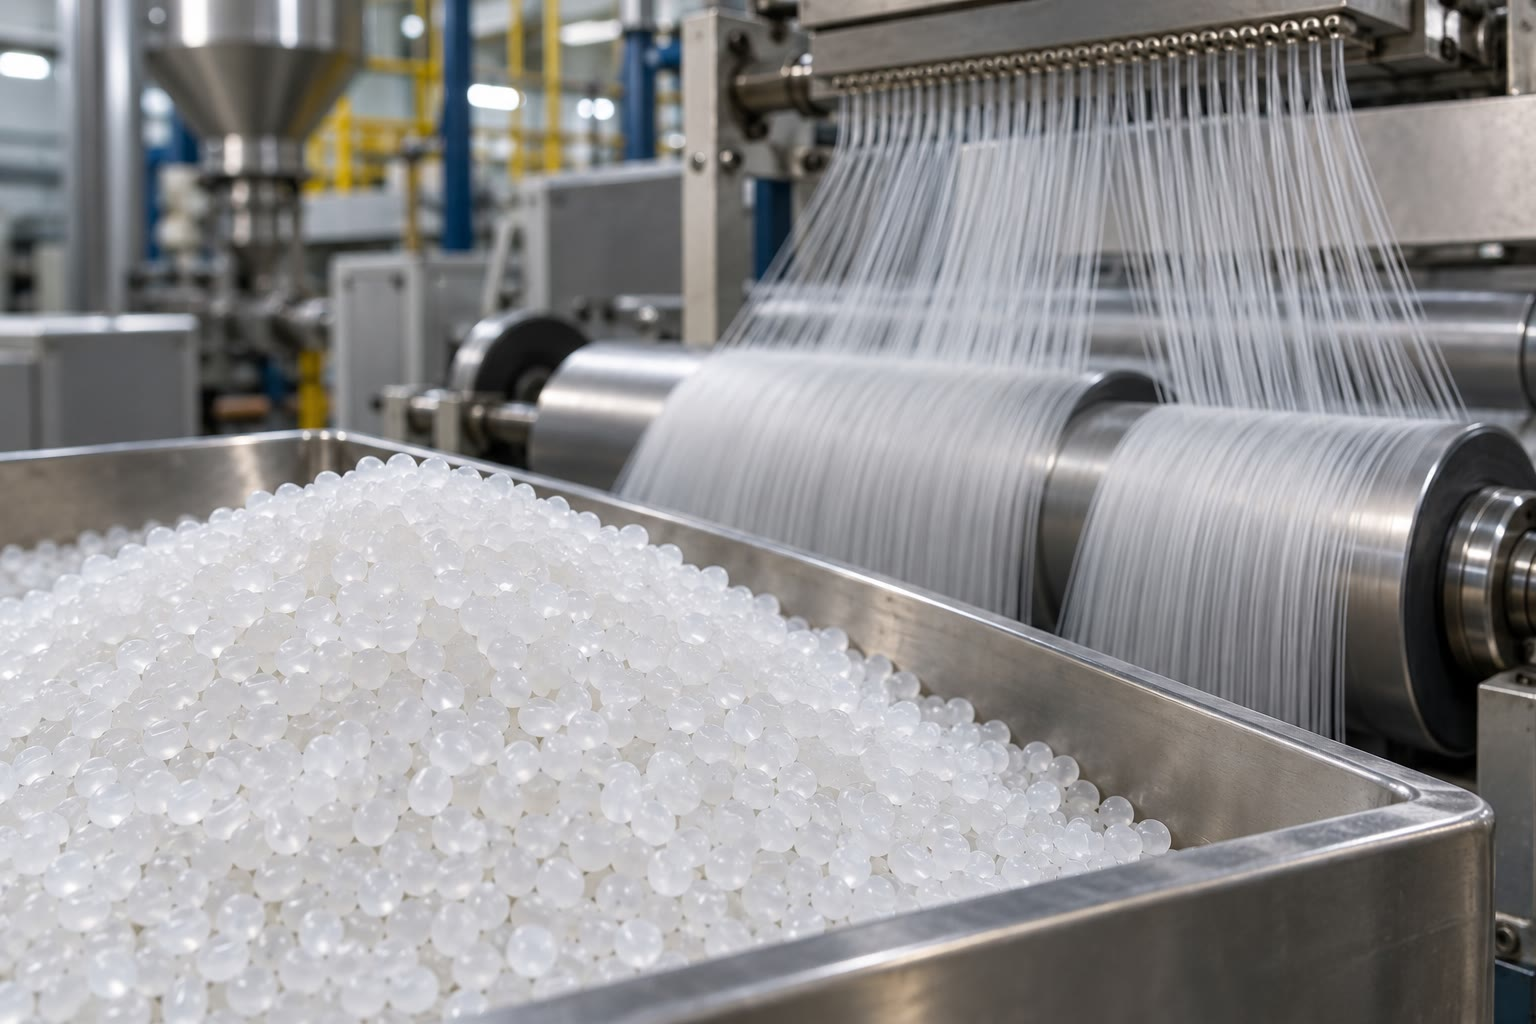
\includegraphics[width=0.58\linewidth]{images/book3/ai/b2-29-pellets.jpg}

{\small \omterm{def:b2:polymer-synthesis:polymer}{Polymer} pellets in a plant, the form in which thermoplastics are sold, and fibres being drawn
from a spinneret onto rotating rolls behind them (illustration).}
\end{omfigure}

\begin{history}[A 99~\% yield is not enough]
\begin{minipage}[t]{0.2\linewidth}
\vspace{0pt}
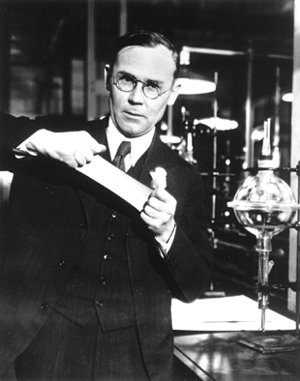
\includegraphics[width=\linewidth]{images/book3/carothers.jpg}
\end{minipage}\hfill
\begin{minipage}[t]{0.76\linewidth}
\vspace{0pt}
Wallace Carothers, a young university instructor recruited into an industrial laboratory for
fundamental research, built long molecules from well-known reactions, and his results strongly
supported the then-contested idea that \omterm{def:b2:polymer-synthesis:polymer}{polymers} are ordinary molecules, only very long. His team
made polyesters, then, from 1934, polyamides; the equation that bears his name explains why only
extreme \omterm{def:b2:continuous-reactors:conversion}{conversions} gave fibres. Nylon went into production in 1939. (Photograph: unknown
photographer, public domain; Wikimedia Commons.)
% ledger: hist:polyamides-1934, hist:nylon-production-1939
\end{minipage}
\end{history}

\begin{safety}{\ghs[5mm]{GHS01}\,\ghs[5mm]{GHS02}\,\ghs[5mm]{GHS05}\,\ghs[5mm]{GHS07}\,\ghs[5mm]{GHS08}\,\ghs[5mm]{GHS09}}
Styrene is flammable and a health hazard. Dibenzoyl peroxide is an explosive oxidiser when dry and is
kept damp and cool. Hexane-1,6-diamine and hexanedioic acid are corrosive to the eyes.
% ledger: ghs:styrene, ghs:BPO, ghs:hexanediamine, ghs:adipic-acid
\end{safety}

\section{Exercises}

\begin{exercise}[$\star$]\label{exo:b2:polymer-synthesis:1}
Draw the \omterm{def:b2:polymer-synthesis:polymer}{repeat units} of polyethene, polypropene, poly(vinyl chloride), polystyrene and nylon-6,6.
\end{exercise}

\begin{exercise}[$\star$]\label{exo:b2:polymer-synthesis:2}
Step or chain growth: PET from ethane-1,2-diol and benzene-1,4-dicarboxylic acid; polystyrene;
nylon-6,6; poly(methyl methacrylate); poly(lactic acid) from 2-hydroxypropanoic acid?
\end{exercise}

\begin{exercise}[$\star$]\label{exo:b2:polymer-synthesis:3}
A polystyrene has $\bar X_n = 1000$. Compute $\bar M_n$, neglecting the end groups.
\end{exercise}

\begin{exercise}[$\star$]\label{exo:b2:polymer-synthesis:4}
A polypropene chain drawn as a planar zig-zag has its methyl groups on the side of the reader, then
away, then towards, then away, and so on. Name its \omterm{def:b2:polymer-synthesis:tacticity}{tacticity}. Could it crystallise?
\end{exercise}

\begin{exercise}[$\star\star$]\label{exo:b2:polymer-synthesis:5}
A sample is a mixture of equal masses of two fractions, of molar masses \qty{10}{kg/mol} and
\qty{100}{kg/mol}. Compute $\bar M_n$, $\bar M_w$ and the \omterm{def:b2:polymer-synthesis:averages}{dispersity}.
\end{exercise}

\begin{exercise}[$\star\star$]\label{exo:b2:polymer-synthesis:6}
Compute $\bar X_n$ for a balanced \omterm{def:b2:polymer-synthesis:step-chain}{step-growth polymerisation} at $p = 0.98$ and $p = 0.995$.
\end{exercise}

\begin{exercise}[$\star\star$]\label{exo:b2:polymer-synthesis:7}
A diacid and a diamine are mixed with a 1~\% excess (in moles) of the diamine. What is the largest
$\bar X_n$ that can be reached?
\end{exercise}

\begin{exercise}[$\star\star$]\label{exo:b2:polymer-synthesis:8}
In a radical polymerisation the initiator concentration is doubled. By what factor do the rate of
polymerisation and the \omterm{def:b2:polymer-synthesis:chain-length}{kinetic chain length} change?
\end{exercise}

\begin{exercise}[$\star\star$]\label{exo:b2:polymer-synthesis:9}
Poly(vinyl chloride) is rigid; garden hoses made of it are flexible because they contain a plasticiser,
a small molecule mixed between the chains. Explain with the glass transition.
\end{exercise}

\begin{exercise}[$\star\star\star$]\label{exo:b2:polymer-synthesis:10}
Show that the Flory mass distribution $w_x = x(1-p)^2p^{\,x-1}$, viewed as a function of a continuous
$x$, is largest at $x = -1/\ln p$, and that this is close to $\bar X_n$ when $p$ is close to 1.
\end{exercise}

\begin{exercise}[$\star\star\star$]\label{exo:b2:polymer-synthesis:11}
PET is made in two stages: dimethyl benzene-1,4-dicarboxylate with excess ethane-1,2-diol gives
bis(2-hydroxyethyl) benzene-1,4-dicarboxylate and methanol; then this diester is heated under vacuum
and polymerises, releasing ethane-1,2-diol. Write both stages and explain how the second stage
solves the stoichiometry problem of the Carothers equation.
\end{exercise}

\begin{exercise}[$\star\star\star$]\label{exo:b2:polymer-synthesis:12}
In a radical copolymerisation of \omterm{def:b2:polymer-synthesis:polymer}{monomers} 1 and 2, the instantaneous composition of the \omterm{def:b2:polymer-synthesis:copolymer}{copolymer} is
given by $\dfrac{\mathrm d[\mathrm M_1]}{\mathrm d[\mathrm M_2]} = \dfrac{[\mathrm M_1](r_1[\mathrm M_1]
+ [\mathrm M_2])}{[\mathrm M_2]([\mathrm M_1] + r_2[\mathrm M_2])}$, where $r_1$ and $r_2$ are the
reactivity ratios (exercise data: $r_1 = 2.0$, $r_2 = 0.5$). Compute the ratio of units in the
\omterm{def:b2:polymer-synthesis:copolymer}{copolymer} formed from an equimolar feed. What happens if $r_1 = r_2 = 0$?
\end{exercise}

\section{Problem: Nylon-6,6 by the Kilogram}

\begin{problem}[{Weekend problem --- the monomers and the nylon salt, the Carothers equation, a
deliberate imbalance, the Flory distribution and the water released}]
\label{pb:b2:polymer-synthesis:1}
Nylon-6,6 is made from hexane-1,6-diamine and hexanedioic acid. End groups are neglected throughout.
Molar masses (\unit{g/mol}): C 12.011, H 1.008, N 14.007, O 15.999.
% ledger: aw:C, aw:H, aw:N, aw:O, ghs:hexanediamine, ghs:adipic-acid

\medskip
\noindent\textbf{Part I --- \omterm{def:b2:polymer-synthesis:polymer}{Monomers} and \omterm{def:b2:polymer-synthesis:polymer}{repeat unit}.}
\begin{enumerate}
  \item Write the formulas of the two \omterm{def:b2:polymer-synthesis:polymer}{monomers}.
  \item Write the equation of the formation of one amide link.
  \item The \omterm{def:b2:polymer-synthesis:polymer}{monomers} are first combined as a 1\,:\,1 salt, crystallised from solution. Why?
  \item Give the \omterm{def:b2:polymer-synthesis:polymer}{repeat unit} of nylon-6,6, its formula and its molar mass.
  \item What is the mean molar mass $M_0$ of a monomer-derived unit in the chain?
  \item What do the two numbers in the name ``6,6'' count?
\end{enumerate}

\medskip
\noindent\textbf{Part II --- The Carothers equation.}
\begin{enumerate}[resume]
  \item Compute $\bar X_n$ and $\bar M_n$ at $p = 0.98$.
  \item The same at $p = 0.99$.
  \item Explain the remark ``a 99~\% yield is not enough''.
  \item Which extent of reaction gives $\bar M_n = \qty{10}{kg/mol}$?
  \item How is the extent pushed so high in practice?
  \item Why must the \omterm{def:b2:polymer-synthesis:polymer}{monomers} be very pure?
\end{enumerate}

\medskip
\noindent\textbf{Part III --- A deliberate imbalance.}
\begin{enumerate}[resume]
  \item The diamine is used in 1~\% molar excess. Compute $r$.
  \item Compute the largest $\bar X_n$ and $\bar M_n$ that can then be reached.
  \item Compute $\bar X_n$ at $p = 0.99$ with this imbalance.
  \item Which groups end the chains at the end of the reaction?
  \item A little ethanoic acid is sometimes added. What does it do to the chains?
  \item Why would a manufacturer limit the chain length on purpose?
\end{enumerate}

\medskip
\noindent\textbf{Part IV --- Distribution and mass balance.}
\begin{enumerate}[resume]
  \item For a balanced mixture at $p = 0.99$, give the \omterm{def:b2:polymer-synthesis:averages}{dispersity}.
  \item Compute $\bar M_w$ at $p = 0.99$.
  \item At $p = 0.99$, what fraction of the molecules, and what fraction of the mass, is still
        unreacted \omterm{def:b2:polymer-synthesis:polymer}{monomer}?
  \item Near which chain length is the mass distribution largest?
  \item Compute the mass of water released per kilogram of nylon-6,6.
  \item Why does melt spinning need $\bar M_n$ within a window?
  \item State the extent of reaction that gives $\bar M_n = \qty{20}{kg/mol}$ for a balanced mixture.
\end{enumerate}
\end{problem}
